\documentclass[a4paper,14pt]{article}
\usepackage{float}
\usepackage{extsizes}
\usepackage{amsmath}
\usepackage{amssymb}
\everymath{\displaystyle}
\usepackage{geometry}
\usepackage{fancyhdr}
\usepackage{multicol}
\usepackage{graphicx}
\usepackage[brazil]{babel}
\usepackage[shortlabels]{enumitem}
\usepackage{cancel}
\usepackage{textcomp}
\usepackage{array}
\usepackage{longtable}
\usepackage{booktabs}
\usepackage{float}   % Para usar o modificador [H]

\columnsep=2cm
\hoffset=0cm
\textwidth=8cm
\setlength{\columnseprule}{.1pt}
\setlength{\columnsep}{2cm}
\renewcommand{\headrulewidth}{0pt}
\geometry{top=1in, bottom=1in, left=0.7in, right=0.5in}

\pagestyle{fancy}
\fancyhf{}
\fancyfoot[C]{\thepage}

\begin{document}
	
	\noindent\textbf{6FMA33 - Matemática} 
	
	\begin{center}Sentenças abertas equivalentes em um universo (Versão estudante)
	\end{center}
	
	\noindent\textbf{Nome:} \underline{\hspace{10cm}}
	\noindent\textbf{Data:} \underline{\hspace{4cm}}
	
	%\section*{Questões de Matemática}
	~ \\
    \begin{multicols}{2}
    	\noindent Dado um conjunto universo U, se duas sentenças abertas têm o mesmo conjunto verdade, dizemos que essas sentenças são \textbf{equivalentes}. \\
    	Para indicar que duas sentenças são equivalentes, usamos o símbolo $ \Leftrightarrow$ entre as sentenças. \\
    	Veja um exemplo:
    	\begin{center}
    		$U = \{2, 3, 4, 5, 6\}$
    	\end{center}
    	A sentença aberta
    	\begin{center}
    		$x - 4 = 0$
    	\end{center}
    	tem conjunto verdade:
    	\begin{center}
    		$V = \{4\}$
    	\end{center}
    	A sentença aberta
    	\begin{center}
    		$x = 4$
    	\end{center}
    	tem conjunto verdade:
    	\begin{center}
    		$V = \{4\}$
    	\end{center}
    	Então, podemos escrever \\
    	 $x - 4 = 0 \Leftrightarrow x = 4$
    	\noindent\textsubscript{~------------------------------------------------------------------------}
    	\begin{enumerate}
    		\item Escreva 5 sentenças abertas e, a partir delas, escreva 5 sentenças abertas com parâmetros.
    		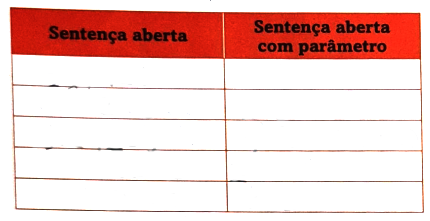
\includegraphics[width=1\linewidth]{imagens_6FMA33/tabela1}
    		\item Em cada item são dados um conjunto universo e duas sentenças abertas. Escreva se são equivalentes ou não e explique.
    		\begin{enumerate}[a)]
    			\item $U = \{2, 3\} ~~~~~ x = 3  ~~~~~ x = 2$ \\\\\\
    			\item $U = \{2, 3, 4\} \\ x - 4 = 0 \\ x = 4$ \\\\\\
    			\item $U = \{0, 1, 2, 3, 4\}$ \\ $x < 3$ \\ $x \leq 2$ \\\\\\
    			\item $U = \left \{ \frac{1}{3}, \frac{1}{4}, \frac{1}{5} \right \}$ \\ $4x - 1 = 0 $ \\ $x = \frac{1}{4}$ \\\\\\
    			\item $U = \mathbb{N} ~~~~~ x = x ~~~~~ 0x = 0$ \\\\\\
    			\item $U = \mathbb{Z} ~~~~~ x^2 = 4 ~~~~~ x = 2$ \\\\\\
    		\end{enumerate}
    	    \item Sendo $U = \mathbb{Z}$, associe as equações com o mesmo conjunto verdade, utilizando o símbolo de equivalência.
    	    \begin{itemize}
    	    	\item $5x = 10$
    	    	\item $-x = 3$
    	    	\item $2x = -12$
    	    	\item $-3x = -21$
    	    	\item $x = 11$
    	    	\item $x = 1$
    	    	\item $x = 7$
    	    	\item $x = 2$
    	    	\item $-2x = 6$
    	    	\item $-x = 12$
    	    	\item $x = -6$
    	    	\item $5x = 5$
    	    \end{itemize}
        	\item Escreva duas sentenças abertas e, a partir delas, escreva duas sentenças abertas com parâmetros.
        	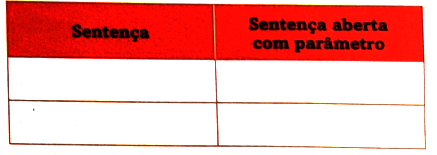
\includegraphics[width=1\linewidth]{imagens_6FMA33/tabela2}
        	\item Em cada item são dados um conjunto universo e duas sentenças abertas. Escreva se são equivalentes ou não e explique.
        	\begin{enumerate}[a)]
        		\item $U = \{1, 2, 3\} \\ x = 3 \\ 3x - 9 = 0$
        		\item $U = \{-2, -1, 0, 1, 2\} \\ x^2 = 4 \\ x(x - 2) = 0$
        	\end{enumerate}
        	\item \begin{enumerate}[a)]
        		\item Resolva a seguinte equação no universo dos inteiros: $-x = 8$ \\\\\\\\\\
        		\item Resolva agora, no mesmo universo, a equação $x = -8$. \\\\
        		\item O que você observou? \\\\
        		\item Qual é a sua conclusão? \\\\
        		\item Será que você poderia \textbf{generalizar} o que você concluir no item acima, ou seja, conseguir algum fato que valha para qualquer valor que um parâmetro possa assumir?
        	\end{enumerate}
        	\item Resolva as inequações abaixo de acordo com o universo dado em cada item. Use equivalências se achar necessário.
        	\begin{enumerate}[a)]
        		\item $U = \{-5, -4, -3\} ~~~~ -x > 3$ \\\\\\\\
        		\item $U = \mathbb{Z} ~~~~ -x > 0$ \\\\\\\\
        		\item $U = \{-6, -4, -2, 2, 4, 6\} \\ -x \leq -4$ \\\\\\\\
        		\item $U = \mathbb{Z} ~~~~ -x \leq 0$
        	\end{enumerate}
    	\end{enumerate}
    $~$ \\ $~$ \\ $~$ \\ $~$ \\ $~$ \\ $~$ \\ $~$ \\ $~$ \\ $~$ \\ $~$ \\ $~$ \\ $~$ \\ $~$ \\ $~$ \\ $~$ \\ $~$ \\ $~$ \\ $~$ \\ $~$ \\ $~$ \\ $~$ \\ $~$ \\ $~$ \\ $~$ \\ $~$ \\ $~$ \\ $~$ \\ $~$ \\ $~$ \\ $~$ \\ $~$ \\ $~$ \\ $~$ \\ $~$ \\ $~$ \\ $~$ \\ $~$ \\ $~$ \\ $~$ \\ $~$ \\ $~$ \\ $~$ \\ $~$ \\ $~$ \\ $~$ \\ $~$ \\ $~$ \\ $~$ \\ $~$ \\ $~$ \\ $~$ \\ $~$ \\ $~$ \\ $~$ \\ $~$ \\ $~$ \\ $~$ \\ $~$ \\ $~$ \\ $~$ \\ $~$ \\ $~$ \\ $~$ \\ $~$ \\ $~$ \\ $~$ \\ $~$ \\ $~$ \\ 
    \end{multicols}
\end{document}